\documentclass[aspectratio=169]{beamer}

\usetheme{Madrid}
\usecolortheme{default}

\usepackage[utf8]{inputenc}
\usepackage[T1]{fontenc}
\usepackage[ngerman]{babel}
\usepackage{amsmath}
\usepackage{listings}
\usepackage{xcolor}
\usepackage{booktabs}
\usepackage{graphicx}
\usepackage{tikz}
\usepackage{hyperref}

\lstset{
  basicstyle=\ttfamily\small,
  keywordstyle=\color{blue},
  commentstyle=\color{gray},
  stringstyle=\color{orange},
  breaklines=true,
  frame=single,
}

% ── Metadata ──────────────────────────────────────────────────────────────────
\title[Automated Data Collection]{Everything, Everywhere, All at Once}
\subtitle{Keynote über das automatisierte Sammeln von Daten}
\author{Stephan Bökelmann}
\institute{PDSC4k – Practical Data Science Conference}
\date{2026}

% ── Document ──────────────────────────────────────────────────────────────────
\begin{document}

% Title slide
\begin{frame}
  \titlepage
\end{frame}

% ── Overview diagram ──────────────────────────────────────────────────────────
\begin{frame}{Die gesamte Reise auf einen Blick}
  \begin{center}
    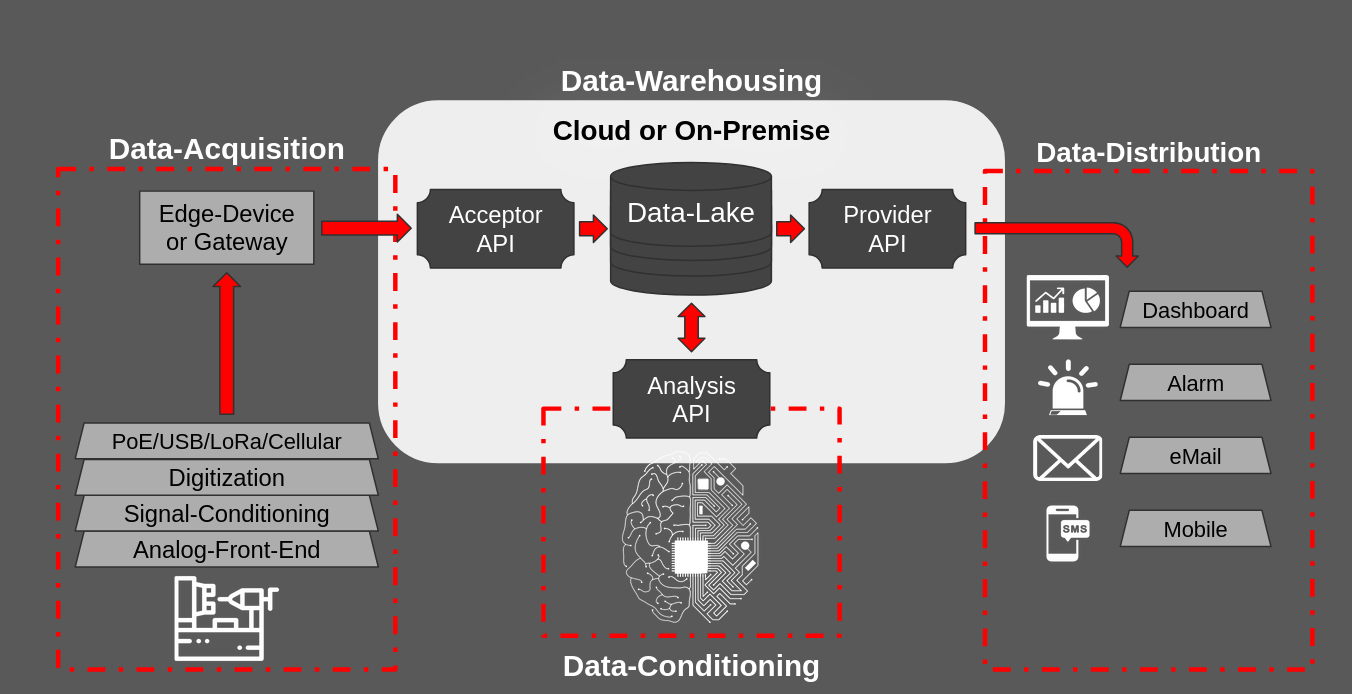
\includegraphics[width=0.92\textwidth]{architecture.png}
  \end{center}
  \vspace{-0.5em}
  \begin{center}
    \small Vier Zonen – eine Verantwortung pro Box.
    Wir gehen sie heute der Reihe nach durch.
  \end{center}
\end{frame}

% Table of contents
\begin{frame}{Agenda}
  \tableofcontents
\end{frame}

% ══════════════════════════════════════════════════════════════════════════════
\section{Data-Acquisition}
% ══════════════════════════════════════════════════════════════════════════════

\begin{frame}{Data-Acquisition: Die physische Welt trifft auf Software}
  \begin{columns}
    \column{0.55\textwidth}
      Die Schichtung von unten nach oben:
      \begin{enumerate}
        \item \textbf{Analog-Front-End} – Verstärkung, Filterung, Impedanz
        \item \textbf{Signal-Conditioning} – Offset, Skalierung, Schutz
        \item \textbf{Digitization} – ADC, Sampling-Rate, Auflösung
        \item \textbf{Transport} – PoE / USB / LoRa / Cellular
        \item \textbf{Gateway} – passiver Netz-Übergang (Modem, LoRa-Basisstation)
        \item \textbf{Edge-Compute} – erster intelligenter Softwareknoten
      \end{enumerate}
    \column{0.4\textwidth}
      \begin{alertblock}{Garbage-in-Problem}
        Fehler in den unteren Schichten sind
        \textbf{nicht} durch spätere Software korrigierbar.
        Ein falsch kalibrierter Sensor liefert
        plausible, aber falsche Daten.
      \end{alertblock}
  \end{columns}
\end{frame}

\begin{frame}{Analog-Front-End und Signal-Conditioning}
  Was hier passiert – und warum es Data Scientists interessieren sollte:
  \begin{itemize}
    \item \textbf{Aliasing}: Sampling-Rate muss $\geq 2\times$ der
          höchsten Signalfrequenz sein (Nyquist)
    \item \textbf{Quantisierungsrauschen}: 12-Bit-ADC $\Rightarrow$
          $\approx 0{,}024\,\%$ Auflösung – reicht das?
    \item \textbf{Offset-Drift}: Temperaturabhängige Verschiebung des
          Nullpunkts $\Rightarrow$ systematischer Fehler
    \item \textbf{Elektromagnetische Störungen}: Differenzmessung,
          Abschirmung, Twisted-Pair
  \end{itemize}
  \vspace{0.5em}
  \begin{exampleblock}{Takeaway}
    Sprich mit den Hardware-Ingenieuren, bevor du das Modell trainierst.
  \end{exampleblock}
\end{frame}

\begin{frame}{Edge-Compute: Gateway und Rechenknoten in einem}
  \begin{columns}
    \column{0.42\textwidth}
      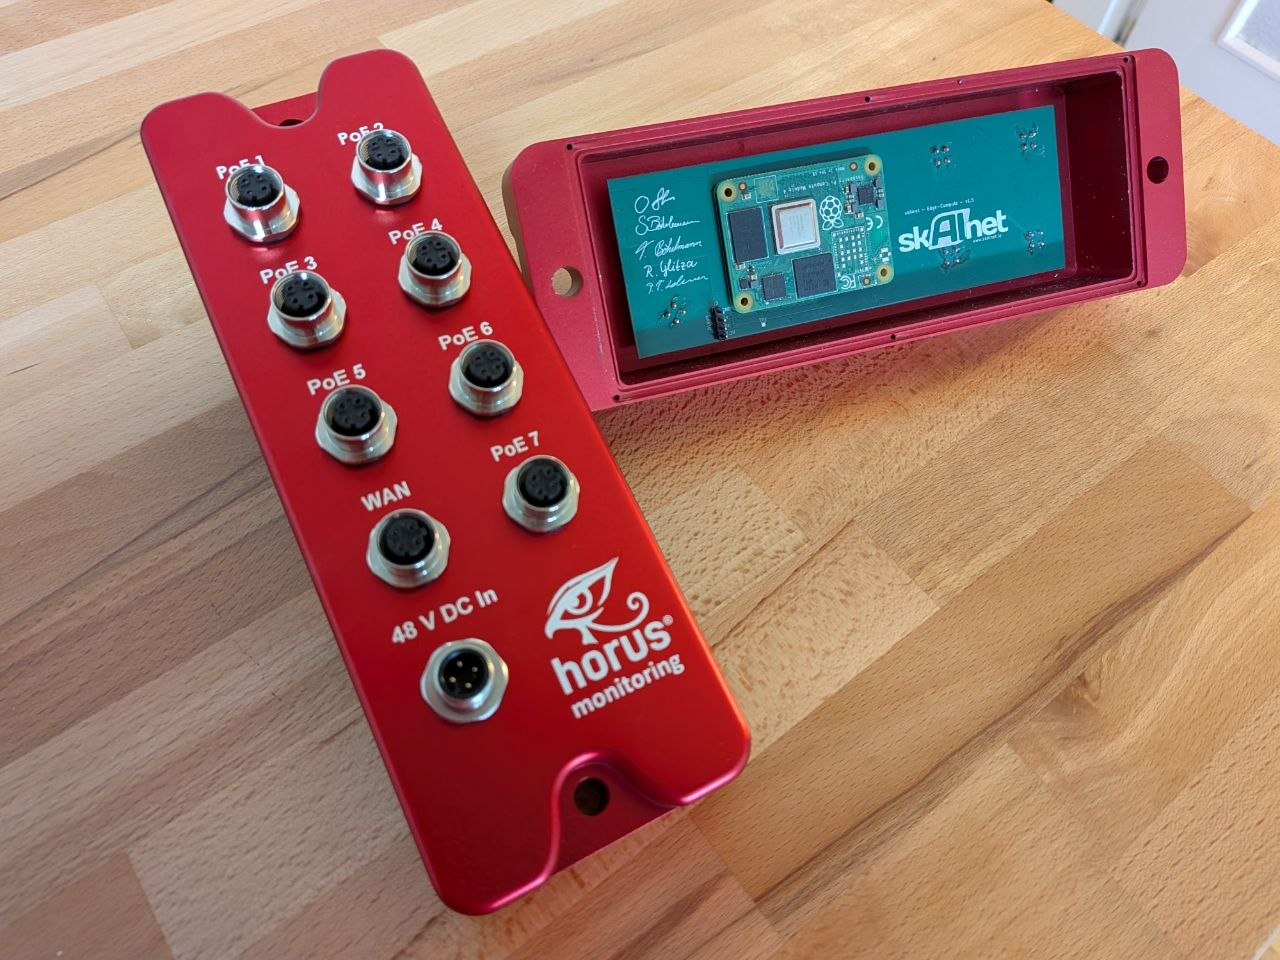
\includegraphics[width=\textwidth]{horus.png}
    \column{0.54\textwidth}
      \textbf{Horus Edge-Compute Platform} (custom mainboard, SBC-agnostisch):
      \begin{itemize}
        \item Integrierter Router mit \textbf{zwei getrennten ETH-Interfaces}
              (WAN / LAN-Isolation)
        \item \textbf{7 PoE-LAN-Ports} – Sensoren werden direkt mitversorgt
        \item \textbf{48\,V DC} Einspeisung, industrietauglich
        \item Sensor-Discovery via \texttt{slook}
              (github: dominicpoeschko) durch den Peripheral-Access-Daemon
        \item Kalibrierung \& Bereinigung \textbf{lokal}, bevor Daten
              über WAN an die Acceptor API weitergehen
        \item Aktuell in Entwicklung: Variante mit \textbf{NVIDIA Jetson}-Modul
              für Inferenz direkt am Edge
      \end{itemize}
  \end{columns}
\end{frame}

\begin{frame}{Warum Compute ans Edge gehört}
  \begin{block}{Unser Architekturmuster}
    Sensoren $\xrightarrow{\text{PoE/LAN}}$ Edge-Compute
    $\xrightarrow{\text{WAN}}$ Acceptor API
  \end{block}
  \vspace{0.5em}
  Was das Edge-Compute \textbf{vor} dem WAN erledigt:
  \begin{enumerate}
    \item \textbf{Aggregation} – Sensordaten beliebig vieler Kanäle bündeln
          (7 PoE-Ports, dahinter beliebig viele Switches)
    \item \textbf{Kalibrierung} – gerätespezifische Korrekturfaktoren anwenden
    \item \textbf{Bereinigung} – Ausreißer, Lücken, Encoding-Fehler
    \item \textbf{Pufferung} – Store-and-forward bei WAN-Ausfall
  \end{enumerate}
  \vspace{0.5em}
  \begin{alertblock}{Faustformel}
    Was \textbf{vor} dem WAN entschieden werden kann, gehört ans Edge –
    Bandbreite ist teuer, Rechenzeit am Edge ist frei.
  \end{alertblock}
\end{frame}

\begin{frame}{Transport-Protokolle im Vergleich}
  \begin{columns}
    \column{0.48\textwidth}
      \begin{block}{Kabelgebunden}
        \begin{itemize}
          \item \textbf{PoE}: Strom + Daten, einfach, zuverlässig
          \item \textbf{USB}: Kurze Distanz, Plug-and-Play
          \item \textbf{Modbus RTU}: Industriestandard, robust
        \end{itemize}
      \end{block}
    \column{0.48\textwidth}
      \begin{block}{Drahtlos}
        \begin{itemize}
          \item \textbf{LoRa}: Lange Reichweite, niedrige Bandbreite
          \item \textbf{Cellular (LTE-M)}: Überall, aber Kosten
          \item \textbf{BLE}: Kurze Distanz, Batterie-freundlich
        \end{itemize}
      \end{block}
  \end{columns}
  \vspace{0.5em}
  \begin{alertblock}{Vergessene Frage}
    Was passiert mit den Daten, wenn die WAN-Verbindung für 3 Stunden ausfällt?
    Store-and-forward am \textbf{Edge-Compute} ist kein Nice-to-have –
    ein passives Gateway puffert nichts.
  \end{alertblock}
\end{frame}

\begin{frame}{Starlink: Satelliteninternet als WAN-Option}
  \begin{columns}
    \column{0.55\textwidth}
      Starlink adressiert den letzten blinden Fleck in der
      Konnektivitätsfrage – \textbf{Standorte ohne Infrastruktur}:
      \begin{itemize}
        \item Latenz aktuell $\approx 20$–$60\,\text{ms}$ (Low-Earth-Orbit)
        \item Bandbreite $\approx 50$–$200\,\text{Mbit/s}$ Down
        \item \textbf{Starlink for IoT}: flaches API-Programm für
              Machine-to-Machine-Kommunikation, optimiert auf
              Dauerbetrieb kleiner Datenpakete
        \item Failover-Option neben LTE-M für kritische Standorte
        \item Hardware: kompaktes Flat-Panel-Dish, wetterfest
      \end{itemize}
    \column{0.4\textwidth}
      \begin{block}{Wann relevant?}
        \begin{itemize}
          \item Bergwerke, Offshore, Baustellen
          \item Landwirtschaft auf großer Fläche
          \item Temporäre Messkampagnen
          \item Backup wenn Cellular ausfällt
        \end{itemize}
      \end{block}
      \begin{alertblock}{Achtung}
        Datenschutz: Serverstandorte
        von Starlink prüfen (DSGVO).
      \end{alertblock}
  \end{columns}
\end{frame}

% ══════════════════════════════════════════════════════════════════════════════
\section{Data-Warehousing}
% ══════════════════════════════════════════════════════════════════════════════

\begin{frame}{Data-Warehousing: Acceptor API $\rightarrow$ Data-Lake}
  \begin{columns}
    \column{0.55\textwidth}
      Die Acceptor API ist das erste Softwaretor:
      \begin{itemize}
        \item Authentifizierung und Autorisierung
        \item Schema-Validierung (Pflichtfelder, Typen)
        \item Rate-Limiting gegen Überflutung
        \item Idempotenz-Schlüssel erzwingen
        \item Schreiben in den Data-Lake (append-only)
      \end{itemize}
    \column{0.4\textwidth}
      \begin{exampleblock}{Designprinzip}
        Die Acceptor API \textbf{lehnt ab oder akzeptiert} –
        sie transformiert nicht.
        Transformation gehört in Data-Conditioning.
      \end{exampleblock}
  \end{columns}
\end{frame}

\begin{frame}{Was landet wirklich im Lake?}
  \begin{columns}
    \column{0.48\textwidth}
      \begin{block}{Gehört rein}
        \begin{itemize}
          \item \textbf{Kalibrierte Messwerte} – vorverarbeitet am Edge
          \item \textbf{Gerätemetadaten} – ID, Firmware, Kalibrierzustand
          \item \textbf{Heartbeats} – Beweis, dass ein Gerät schweigt
        \end{itemize}
      \end{block}
    \column{0.48\textwidth}
      \begin{alertblock}{Gehört \textbf{nicht} rein}
        \begin{itemize}
          \item Polling-Artefakte ohne Messwert
          \item Duplikate durch Retry (filtern, nicht speichern)
          \item Interne Diagnosedaten des Edge-Compute
        \end{itemize}
      \end{alertblock}
  \end{columns}
  \vspace{0.5em}
  \begin{exampleblock}{Faustregel}
    Alles, was nötig ist, um den Zustand der Welt
    \textbf{zum Messzeitpunkt rekonstruieren} zu können – nicht mehr, nicht weniger.
  \end{exampleblock}
\end{frame}


\begin{frame}{Praxis: Ceph als echte Cloud-Lösung – mit der THGA}
  \begin{columns}
    \column{0.48\textwidth}
      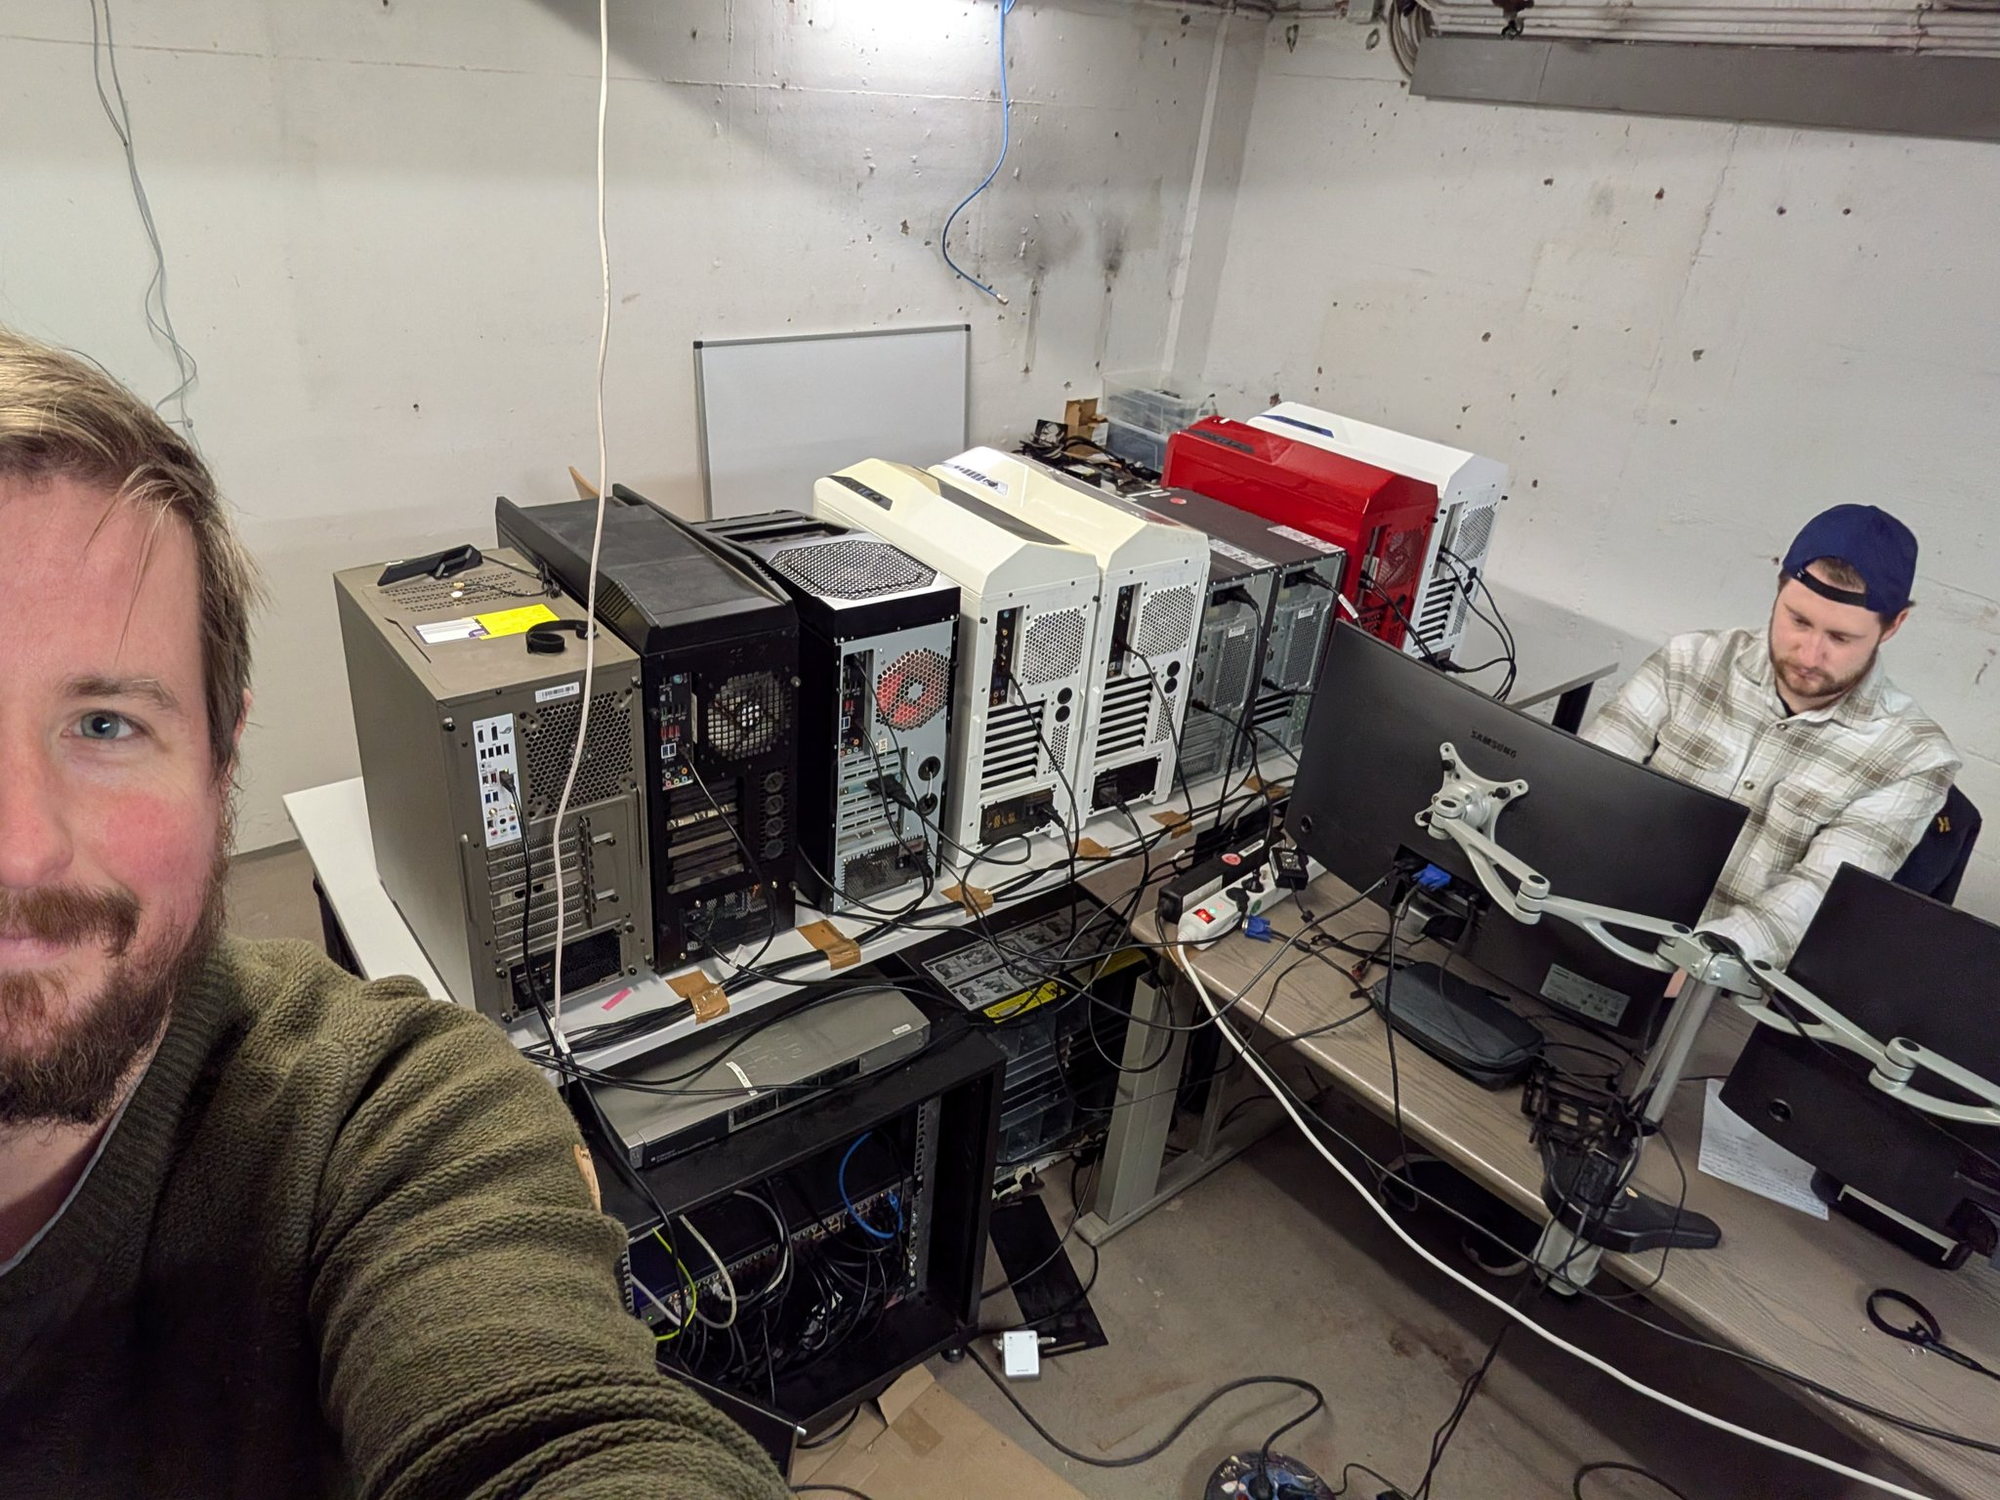
\includegraphics[width=\textwidth]{ceph.png}
    \column{0.48\textwidth}
      Philipp Lehmann und ich haben gemeinsam mit der
      \textbf{Technischen Hochschule Georg Agricola (THGA)}
      eine vollständige Cloud-Infrastruktur auf Ceph-Basis aufgebaut –
      kein Proof-of-Concept mehr, sondern \textbf{produktiv in Betrieb}:
      \begin{itemize}
        \item Aktuell \textbf{100\,TB nutzbar} – wird weiter ausgebaut
        \item Echte Fehlerfälle produziert und analysiert
        \item Paper in Vorbereitung
      \end{itemize}
      \vspace{0.5em}
      \begin{exampleblock}{}
        Philipp ist heute hier –
        sprecht ihn an, er kann mehr dazu erzählen.
      \end{exampleblock}
  \end{columns}
\end{frame}

\begin{frame}{IPFS als Storage-Backend hinter dem Acceptor}
  \begin{columns}
    \column{0.55\textwidth}
      \textbf{Architektur:}
      \begin{enumerate}
        \item Acceptor schreibt Daten $\rightarrow$ \textbf{IPFS-Node}
        \item IPFS gibt \textbf{CID} zurück (Content Identifier = Hash)
        \item CID + Metadaten $\rightarrow$ \textbf{On-Premise Metadaten-DB}
        \item \textbf{FastAPI-Katalog} gibt nur Metadaten \& CID aus
        \item Consumer holt Daten selbst per CID aus IPFS
      \end{enumerate}
    \column{0.4\textwidth}
      \begin{block}{Warum IPFS?}
        \begin{itemize}
          \item CID ist Prüfsumme – kein Silent Corruption
          \item Unveränderlichkeit by design
          \item Deduplizierung gratis
          \item Speicherort austauschbar (Ceph, S3, Cluster)
        \end{itemize}
      \end{block}
      \begin{alertblock}{Trennung}
        Metadaten bleiben On-Premise
        oder in separater Cloud –
        nie zusammen mit den Daten.
      \end{alertblock}
  \end{columns}
\end{frame}

\begin{frame}{Cloud vs. On-Premise: Eine echte Entscheidung}
  \begin{columns}
    \column{0.48\textwidth}
      \begin{block}{Cloud}
        \begin{itemize}
          \item Elastische Skalierung
          \item Kein Betrieb von Hardware
          \item Pay-per-use (Achtung: Egress-Kosten!)
          \item DSGVO: Serverstandort beachten
        \end{itemize}
      \end{block}
    \column{0.48\textwidth}
      \begin{block}{On-Premise}
        \begin{itemize}
          \item Datensouveränität
          \item Planbare Fixkosten
          \item Luftspalt für kritische Systeme
          \item Betriebsaufwand intern
        \end{itemize}
      \end{block}
  \end{columns}
  \vspace{0.5em}
  \begin{alertblock}{Hybride Realität}
    Acquisition on-premise, Warehousing in der Cloud – das ist der häufigste
    Kompromiss in der Industrie.
  \end{alertblock}
\end{frame}

\begin{frame}{Backpressure: Was passiert, wenn alle gleichzeitig senden?}
  \begin{alertblock}{Das Szenario}
    50 Edge-Computes schicken nach einem WAN-Ausfall gleichzeitig
    ihre gepufferten Daten – die Acceptor API wird geflutet.
  \end{alertblock}
  \vspace{0.5em}
  \begin{columns}
    \column{0.32\textwidth}
      \textbf{Drosseln (Acceptor):}
      \begin{itemize}
        \item \textbf{Token Bucket} – Durchsatz pro Client
        \item \textbf{Circuit Breaker} – \texttt{503} bei Überlast
        \item \textbf{Sliding Window} – Burst ok, Dauerfeuer nicht
      \end{itemize}
    \column{0.32\textwidth}
      \textbf{Skalieren (Infrastruktur):}
      \begin{itemize}
        \item \textbf{k8s HPA} – neue Acceptor-Pods bei Last
        \item \textbf{Load Balancer} – verteilt auf Pod-Pool
        \item Zustandslos designen – jeder Pod gleich
      \end{itemize}
    \column{0.32\textwidth}
      \textbf{Puffern (Edge-Compute):}
      \begin{itemize}
        \item \texttt{503} $\Rightarrow$ Backoff + Jitter
        \item Lokaler Puffer wartet
        \item Frische Daten zuerst
      \end{itemize}
  \end{columns}
  \vspace{0.5em}
  \begin{exampleblock}{Kernidee}
    Drosseln und Skalieren schließen sich nicht aus –
    beides zusammen ergibt ein robustes System.
  \end{exampleblock}
\end{frame}

% ══════════════════════════════════════════════════════════════════════════════
\section{Data-Conditioning}
% ══════════════════════════════════════════════════════════════════════════════

\begin{frame}{Data-Conditioning: Wo Daten denken lernen}
  \begin{center}
    Die bidirektionale Verbindung im Diagramm ist kein Zufall:
  \end{center}
  \vspace{0.5em}
  \begin{columns}
    \column{0.48\textwidth}
      \textbf{Lake $\rightarrow$ Analysis API}
      \begin{itemize}
        \item Rohdaten lesen
        \item Bereinigen, Normalisieren
        \item Feature-Engineering
        \item Modell-Inferenz
      \end{itemize}
    \column{0.48\textwidth}
      \textbf{Analysis API $\rightarrow$ Lake}
      \begin{itemize}
        \item Abgeleitete Features zurückschreiben
        \item Annotationen, Labels
        \item Modell-Outputs als neue Datensätze
        \item Aggregierte Sichten für Distribution
      \end{itemize}
  \end{columns}
  \vspace{0.5em}
  \begin{exampleblock}{Schlüsselidee}
    Conditioning \textbf{schreibt zurück} – der Lake wächst durch Analyse.
  \end{exampleblock}
\end{frame}

\begin{frame}{Analyse über einen FastAPI-Datenkatalog}
  \begin{columns}
    \column{0.55\textwidth}
      Statt Daten auszuliefern gibt der Katalog nur \textbf{Metadaten}:
      \begin{itemize}
        \item Welche Datensätze existieren?
        \item CID / Speicherort in IPFS
        \item Zeitraum, Gerät, Kalibrierzustand
        \item Qualitätsstatus (validiert / nicht validiert)
      \end{itemize}
      \vspace{0.5em}
      Der Consumer entscheidet selbst, was er lädt –
      der Katalog transportiert keine Nutzdaten.
    \column{0.4\textwidth}
      \begin{block}{Vorteile}
        \begin{itemize}
          \item Kein zentraler Flaschenhals
          \item Reproduzierbarkeit: CID = exakte Datenversion
          \item Zugriffskontrolle auf Metadaten-Ebene
          \item FastAPI: schnell, typsicher, OpenAPI gratis
        \end{itemize}
      \end{block}
      \begin{exampleblock}{}
        \texttt{GET /datasets?device=T42\&from=2026-01-01}\\
        \texttt{→ \{cid, location, quality\}}
      \end{exampleblock}
  \end{columns}
\end{frame}

\begin{frame}{Orchestrierung der Conditioning-Pipelines}
  Der Orchestrator läuft auf dem \textbf{Analyse-Rechner} –
  nicht im Warehouse. Er fragt den FastAPI-Katalog nach CIDs,
  lädt Daten aus IPFS und schreibt Ergebnisse zurück.
  \vspace{0.3em}

  Was Orchestratoren leisten:
  \begin{itemize}
    \item Cron-ähnliches Scheduling mit Abhängigkeitsgraphen (DAGs)
    \item Automatischer Retry mit konfigurierbaren Policies
    \item Backfill: fehlende Zeitscheiben nachträglich verarbeiten
    \item Alerting bei Failure, SLA-Verletzung
    \item Audit-Log über jeden Pipeline-Run
  \end{itemize}
  \vspace{0.5em}
  \begin{tabular}{ll}
    \toprule
    \textbf{Tool} & \textbf{Stärke} \\
    \midrule
    Apache Airflow & Mature, große Community, komplex \\
    Prefect        & Python-nativ, einfach zu starten \\
    dbt            & SQL-fokussiert, Transformations-Layer \\
    \bottomrule
  \end{tabular}
\end{frame}


% ══════════════════════════════════════════════════════════════════════════════
\section{Data-Distribution}
% ══════════════════════════════════════════════════════════════════════════════

\begin{frame}{Data-Distribution: Wer bekommt was, wann, wie?}
  \begin{columns}
    \column{0.55\textwidth}
      Die Provider API ist die \textbf{vertragliche Grenze}
      nach außen:
      \begin{itemize}
        \item Versionierung (v1, v2 – nicht breaking)
        \item \textbf{Keycloak} – OIDC / OAuth2, rollenbasiert, SSO-fähig
        \item Rate-Limiting pro Consumer
        \item Dokumentation (OpenAPI / AsyncAPI)
      \end{itemize}
    \column{0.4\textwidth}
      \begin{block}{Vier Consumer-Typen}
        \begin{itemize}
          \item Dashboard (Pull, niedrige Latenz)
          \item Alarm (Push, Echtzeit)
          \item eMail (asynchron, gebündelt)
          \item Mobile (Push-Notification)
        \end{itemize}
      \end{block}
  \end{columns}
\end{frame}

\begin{frame}{Provider API: FastAPI oder Crow/C++ – und was kostet das SLA?}
  \begin{columns}
    \column{0.48\textwidth}
      \textbf{Technologiewahl nach Last:}
      \begin{tabular}{lll}
        \toprule
        & \textbf{FastAPI} & \textbf{Crow (C++)} \\
        \midrule
        Aufbau    & Stunden  & Tage \\
        Latenz    & $\sim$5\,ms & $<$1\,ms \\
        Durchsatz & $\sim$10k\,req/s & $>$100k\,req/s \\
        Betrieb   & einfach  & komplex \\
        \bottomrule
      \end{tabular}
      \vspace{0.5em}
      Faustregel: unter $\sim$20k\,req/s ist FastAPI die
      richtige Wahl – darüber lohnt C++.
    \column{0.48\textwidth}
      \textbf{Was das SLA konkret bedeutet:}
      \begin{itemize}
        \item \textbf{Verfügbarkeit}: z.\,B. 99,9\,\% = max.\ 8,7\,h
              Ausfall/Jahr – wer zahlt darunter?
        \item \textbf{Latenz}: p99 $<$ 200\,ms – nicht Mittelwert,
              sondern Worst-Case-Perzentil
        \item \textbf{Freshness}: Daten maximal $X$ Minuten alt
      \end{itemize}
      \vspace{0.3em}
      \begin{block}{k8s als Hebel}
        HPA skaliert Provider-Pods bei Last –
        SLA-Ziele werden durch Skalierung,
        nicht durch Überdimensionierung gehalten.
      \end{block}
  \end{columns}
\end{frame}

\begin{frame}{Latenz- und Formatanforderungen je Consumer}
  \begin{tabular}{lllll}
    \toprule
    \textbf{Consumer} & \textbf{Latenz} & \textbf{Format} &
    \textbf{Mechanismus} & \textbf{Priorität} \\
    \midrule
    Dashboard  & $<1\,s$    & JSON / REST    & Polling / WebSocket & Mittel \\
    Alarm      & $<100\,ms$ & Minimal        & Webhook / MQTT      & Kritisch \\
    eMail      & Minuten    & HTML / Text    & Queue               & Niedrig \\
    Mobile     & $<5\,s$    & FCM / APNs     & Push-Notification   & Hoch \\
    \bottomrule
  \end{tabular}
  \vspace{0.5em}
  \begin{alertblock}{Wichtig}
    Ein einziger API-Endpunkt für alle Consumer ist ein Anti-Pattern.
    Latenzanforderungen sind zu verschieden.
  \end{alertblock}
\end{frame}

\begin{frame}{Alarmierung richtig gemacht}
  Häufige Fehler bei Alarmsystemen:
  \begin{itemize}
    \item \textbf{Alert-Fatigue}: Zu viele Alarme $\Rightarrow$ alle werden ignoriert
    \item \textbf{Keine Hysterese}: Schwellwert-Flattern erzeugt Alarm-Storms
    \item \textbf{Falscher Empfänger}: Alarm geht an alle, niemand fühlt sich zuständig
    \item \textbf{Kein Kontext}: Alarm ohne Messwert, Trend, oder Handlungsanweisung
  \end{itemize}
  \vspace{0.5em}
  \begin{exampleblock}{Guter Alarm}
    »Sensor T-42 überschreitet $85\,°C$ seit 3 Minuten (aktuell $91\,°C$,
    Trend: steigend). Verantwortlich: On-Call Mechanik. Runbook: \texttt{/wiki/T42}«
  \end{exampleblock}
\end{frame}

\begin{frame}{Trennung der Verantwortlichkeiten: Alarm, Analyse, Warehouse}
  \begin{alertblock}{Anti-Pattern: alles auf einem Rechner}
    Wenn Warehouse, Analyse und Alarmierung dieselbe Infrastruktur teilen,
    zieht ein Ausfall alle drei gleichzeitig mit – genau dann, wenn
    Alarme am wichtigsten wären.
  \end{alertblock}
  \vspace{0.5em}
  \begin{columns}
    \column{0.48\textwidth}
      \textbf{Drei getrennte Systeme:}
      \begin{itemize}
        \item \textbf{Warehouse} – Acceptor, Lake, Provider API
        \item \textbf{Analyse} – Conditioning, FastAPI-Katalog,
              ML-Pipelines
        \item \textbf{Alarm-Service} – eigenständiger Rechner,
              sendet eMail / SMS / Push unabhängig
      \end{itemize}
    \column{0.48\textwidth}
      \begin{block}{Tradeoff}
        Höherer Ersteinrichtungsaufwand –\\
        aber jede Komponente ist einzeln\\
        wartbar, skalierbar und ersetzbar.
      \end{block}
      \begin{exampleblock}{Meta-Monitoring}
        \textbf{Uptime Kuma} (o.\,ä.) überwacht
        das Warehouse von außen –
        Monitoring des Monitorings.
        Wer wacht über den Wächter?
      \end{exampleblock}
  \end{columns}
\end{frame}

% ══════════════════════════════════════════════════════════════════════════════
\section{Das Diagramm als Checkliste}
% ══════════════════════════════════════════════════════════════════════════════

\begin{frame}{Jede Box ist eine Verantwortungsgrenze}
  \begin{center}
    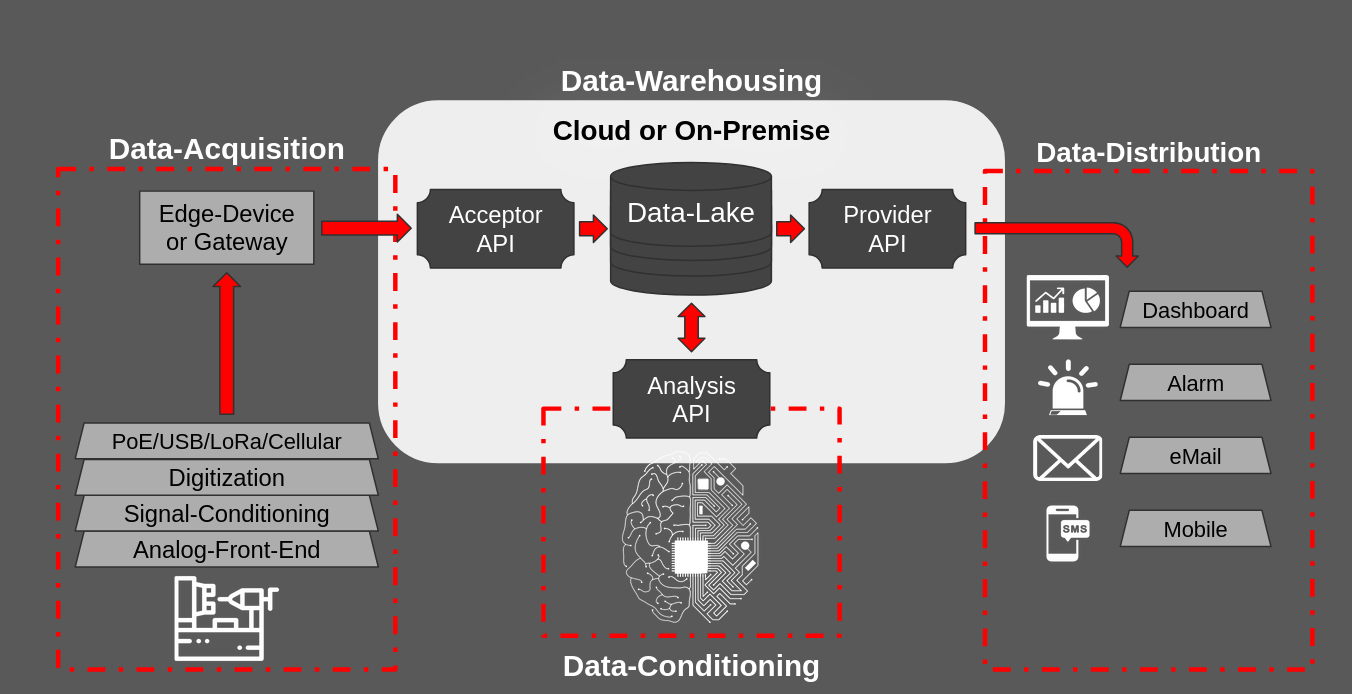
\includegraphics[width=0.82\textwidth]{architecture.png}
  \end{center}
  \vspace{-0.3em}
  \begin{center}
    \small Wer \textbf{besitzt} welche Box in eurer Organisation?
  \end{center}
\end{frame}

\begin{frame}{Checkliste: Ist eure Pipeline production-ready?}
  \begin{columns}
    \column{0.48\textwidth}
      \textbf{Data-Acquisition}
      \begin{itemize}
        \item[$\square$] Kalibrierung dokumentiert?
        \item[$\square$] Store-and-forward am Edge?
        \item[$\square$] Verbindungsabbruch getestet?
      \end{itemize}
      \textbf{Data-Warehousing}
      \begin{itemize}
        \item[$\square$] Acceptor idempotent?
        \item[$\square$] Rohdaten unveränderlich gespeichert?
        \item[$\square$] \texttt{last\_write\_timestamp} gemonitort?
      \end{itemize}
    \column{0.48\textwidth}
      \textbf{Data-Conditioning}
      \begin{itemize}
        \item[$\square$] Quality Gates vor jeder Transformation?
        \item[$\square$] Backfill-Strategie dokumentiert?
        \item[$\square$] Abgeleitete Daten versioniert?
      \end{itemize}
      \textbf{Data-Distribution}
      \begin{itemize}
        \item[$\square$] Provider API versioniert?
        \item[$\square$] Alarm-Hysterese konfiguriert?
        \item[$\square$] Consumer-Latenz getestet?
      \end{itemize}
  \end{columns}
\end{frame}

\begin{frame}{Fazit: Drei Sätze zum Mitnehmen}
  \begin{enumerate}
    \item \textbf{Daten sammeln ist Engineering} –
          nicht ein Skript, das irgendwo läuft und hofft.
    \item \textbf{Qualität entsteht an der Quelle} –
          was das Analog-Front-End verdirbt, rettet kein Modell.
    \item \textbf{Jede Box braucht einen Besitzer} –
          die größte Datenpipeline scheitert an ungeklärter Verantwortung,
          nicht an Technologie.
  \end{enumerate}
\end{frame}

% ── Closing slide ─────────────────────────────────────────────────────────────
\begin{frame}
  \begin{center}
    {\Huge \textbf{Jetzt seid ihr dran.}}\\[1em]
    {\large Baut Pipelines, die nicht lügen.}\\
    {\large Viel Spaß auf der PDSC4k – und einen guten Austausch!}\\[2em]
    \textbf{Stephan Bökelmann}\\
    \texttt{stephan.boekelmann@gruppe.ai}\\[1em]
    \small
    \texttt{github.com/maxclerkwell/pdsc4k-talk}\\[0.4em]
    Kooperation: \texttt{www.skAInet.io}\\
    Blog: \texttt{maxclerkwell.github.io}
  \end{center}
\end{frame}

\end{document}
